\documentclass{article}
\usepackage{graphicx}
\usepackage{amsmath}
\usepackage{float}
\usepackage{booktabs, 
            makecell, multirow, tabularx}
\usepackage{xcolor}

\title{derivative's}

\begin{document}


\section{Defining average and instantaneous rates of change at a point}
\subsection{Derivative as a concept:}
\noindent
    Derivative is defined as the instantaneous rate of change at a point, 
    or the slope of a tangent line at that point.\\
    which is defined as the \(\lim_{x\to0}\frac{dy}{dx} = f'(x)\).
\subsection{Secant lines and average rate of change:}
    the average rate of change between two points in an interval $[a, b]$ of a curve is defined as the slope of the secant line that connects these points.\newline \newline
    example: \newline \newline

\begin{figure}[ht]
    \centering
    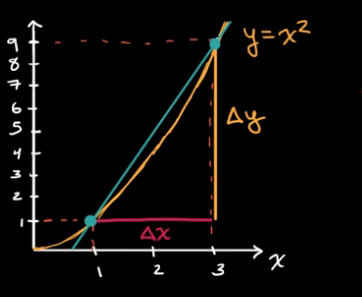
\includegraphics[bb=0 0 360 297, width=0.7\textwidth]{images/secant_line.png}
    \caption{secant line}\label{fig:secant line} 
\end{figure}


\section{Defining the derivative of a function and using derivative notation}
\subsection{Formal definition of the derivative as a limit:}
    h represent some distance more than x. 
    the derivative of a point \(x_0\) formally defined as 
    
   \large \[f'(x_0) = \lim_{h\to0}\hspace{4pt}\frac{f(x_0 + h) - f(x_0)}{h}\]

\subsection{Alternate form of the derivative: }
    the derivative of a point \(x_0\) in alternate form is written as
    
    \large \[f'(x_0) = \lim_{x\to x_0}\hspace{4pt}\frac{f(x) - f(x_0)}{x - x_0}\]
\section{Connecting differentiability and continuity}
\subsection{Differentiability and continuity}
    \begin{itemize}
        \item if f (x) is differentiable at \(x = c\), then f (x) is continuous at \(x = c\)
        \item if f (x) is not continuous at \(x = c\), then f (x) is not differentiable at \(x = c\)
        \item if f (x) is not differentiable at a point, then f (x) may or may not be continuous at that point.
    \end{itemize}
\section{Power rule}
    let the function \large \(f(x) = x ^ n, n\neq 0\), the derivative of \(f(x)\) is given according to the power rule as \large \[f'(x) = nx^{n-1}\]
\section{Derivative rules: constant, sum, difference and constant multiple}
\subsection{Basic rules}
    \begin{itemize}
        \item let A be a constant then \(\frac{d}{dx}[A] = 0\).
        \item let \(f(x)\) be a defined function then: \[\frac{d}{dx}[Af(x)] = A\frac{d}{dx}[f(x)] = Af'(x)\]
        \item let g (x) be a defined function then: \[\frac{d}{dx}[f(x) + g(x)] = \frac{d}{dx}[f(x)] + \frac{d}{dx}[g(x)] = f'(x) + g'(x)\]
    \end{itemize}

\section{Derivatives of \(\cos(x)\), \(\sin(x)\), \(e^x\) and \(\ln (x)\)}
\subsection{Derivatives of \(\sin(x)\) and \(\cos(x)\)}
    \begin{itemize}
        \item \(\frac{d}{dx}[\sin(x)] = \cos(x)\)
        \item \(\frac{d}{dx}[\cos(x)] = -\sin(x)\)
    \end{itemize}
\subsection{Derivative of \(e^x\)}
    \(\frac{d}{dx}[e^x] = e ^ x\)
\subsection{Derivative of \(\ln (x)\)}
    \(\frac{d}{dx}[\ln (x)] =\frac{1}{x}\)
\section{The product rule}
    \[\frac{d}{dx}[f(x)g(x)] = f'(x)g(x) + f(x)g'(x)\]
\section{The Quotient rule}
    \[\frac{d}{dx}\left[\frac{f(x)}{g(x)}\right] = \frac{\frac{d}{dx}[f(x)] \cdot g(x) - f(x) \cdot \frac{d}{dx}[g(x)]}{{g(x)}^2}\]
\section{Derivatives of  \(\tan(x)\) and \(\cot(x)\)}
    tan (x): 
        \[\frac{d}{dx}[\tan(x)] = \frac{d}{dx} \left[ \frac{\sin(x)}{\cos(x)} \right] = \frac{\cos(x) \cdot \cos(x) + \sin(x) \cdot \sin(x) }{\cos{x}^2 } = \frac{1}{\cos{x}^2} = \sec{x}^2 \]
    cot (x): 
        \[\frac{d}{dx}[\cot(x)] = \frac{d}{dx} \left[ \frac{\cos(x)}{\sin(x)} \right] = \frac{-\sin(x) \cdot \sin(x) - \cos(x) \cdot \cos(x) }{\sin{x}^2 } = -\frac{1}{\sin{x}^2} = -\csc{x}^2 \]
\section{Chain rule}
      \[\frac{d}{dx}[f\Bigl(g(x)\Bigr)] = f'\Bigl(g(x)\Bigr) \cdot g'(x)\]
\section{The chain rule: further practice}
    \subsection{Derivative of \(a^x\)(for any positive base a)}
    let \(a = e^{\ln a}\) then: 
    
    \[\frac{d}{dx}[a^x] = \frac{d}{dx}\Bigl[{\Bigl(e^{\ln a} \Bigr)}^{x}\Bigr] = e^{(\ln a)\cdot x} \cdot \ln a = (\ln a) \cdot a^{x}\] 

    \subsection{Derivative of \( \log_a x\) (for any positive base \(a \neq 1\))}
    let \(\frac{d}{dx}[\ln x] = \frac{1}{x}\) and \(\log_a b = \frac{\log_c b}{\log_c a}\) then: 
    \[\frac{d}{dx}[\log_a x] = \frac{d}{dx}\Bigl[\frac{1}{\ln a} \cdot \ln x \Bigr] = \frac{1}{\ln a} \cdot \frac{d}{dx}[\ln x] = \frac{1}{(\ln a)x} \] 
    \subsection{Proving the chain rule}
        \begin{itemize}
            \item \(u(x)\) continuous at \(x = c\) implies that \(\Delta u \to 0\) as \(\Delta x \to 0\)
            \item \(u(x)\) is continuous \(\iff \lim_{x \to c} u(x) = u(c) \equiv \lim_{x \to c}(u(x) - u(c)) = 0\) 
        \end{itemize}
        we have: 
        \begin{itemize}
            \item \(\Delta u = u(x) - u(c)\)
            \item  \(\Delta x = x - c\)
            \item \(\lim_{\Delta x \to 0} \Delta u = 0\)
        \end{itemize}

        \begin{figure}[ht]
            \centering
            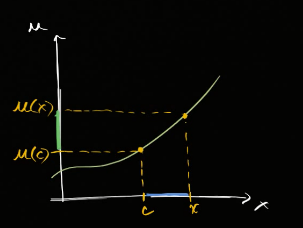
\includegraphics[bb=0 0 303 228, width=0.7\textwidth]{images/change_x_change_u_continuous.png}
            \caption{if function u is continuous at x, then \(\Delta u \to 0\) as \(\Delta x \to 0\)}\label{fig:change_x_change_u_continuous}
        \end{figure}
        chain rule prove: 
        
        assume y, u differentiable at x.
        \[\frac{d}{dx}[y(u(x))] = \frac{dy}{dx} = \frac{dy}{dy} \cdot \frac{dy}{dx}\]
        \[\frac{dx}{dy} = \lim_{\Delta x \to 0} \frac{\Delta y}{ \Delta x} = \lim_{\Delta x \to 0} \frac{\Delta y}{\Delta u} \cdot \frac{\Delta u}{\Delta x} =  \Bigl(\lim_{\Delta x \to 0} \frac{\Delta y}{\Delta u} \Bigr) \cdot \Bigl(\lim_{\Delta x \to 0} \frac{\Delta u}{\Delta x} \Bigr) \]
        \[= \Bigl(\lim_{\Delta u \to 0} \frac{\Delta y}{\Delta u} \Bigr) \cdot \frac{du}{dx} = \frac{dy}{dy} \cdot \frac{du}{dx}\]
        \subsection{Implicit differentiation}
            In implicit differentiation, we differentiate each side of an equation with two variables, by treating one of the variables as function of the other.this calls for using chain rule.

            \noindent example differentiating \(x^2 + y^2 = 1\): 

            \noindent we treat y as an implicit function of x 

            \[x^2 + y^2 = 1\]
            \[\frac{d}{dx}(x^2 + y^2) = \frac{d}{dx}(1)\]
            \[\frac{d}{dx}(x^2) +\frac{d}{dx}(y^2) = 0\]
            \[2x + 2y \cdot \frac{dy}{dx} = 0\]
            \[2y \cdot \frac{dy}{dx} = -2x\]
            \[ \frac{dy}{dx} = -\frac{x}{y}\]
        \subsection{Differentiating inverse functions}
            let f (x) a defined function \noindent
            let g (x) be \(g(x) = f^{-1}(x)\) then \(g(f(x)) = x\) and 
            \[\frac{d}{dx}[g(f(x))] = \frac{d}{dx}[x]\]
            \[g'(f(x)) \cdot f'(x) = 1\]
            \[f'(x) = \frac{1}{g'(f(x))}\]
        \subsection{Differentiating inverse trigonometric functions}
            let \[\sin^2 y + \cos^2 y = 1\]
            Inverse sine:\\
                let \(x = \sin y \)
                \[y = \sin^{-1} x\]
                \[\frac{d}{dx}[\sin y ] = \frac{d}{dx}[x]\]
                \[\cos y \cdot \frac{dy}{dx} = 1 \]
                \[\frac{dy}{dx} = \frac{1}{\cos y}\]
                \[= \frac{1}{\sqrt{1 - {(\sin y)}^2}}\]
                \[\frac{d}{dx}[\sin^{-1}(x)] = \frac{1}{\sqrt{1 - x^2}}\]
            Inverse cosine:\\ 
            let \(x = \cos y\) 
                \[y = \cos^{-1} x\]
                \[1 = (-\sin y)\frac{dy}{dx}\]
                \[\frac{dy}{dx} = - \frac{1}{\sin y} = -\frac{1}{\sqrt{1 - P{(\cos y)}^2}} = - \frac{1}{\sqrt{1 - x^2}}\]
                \[\frac{d}{dx}[\cos^{-1} x] = -\frac{1}{\sqrt{1 - x^2}}\]
            Inverse tangent:\\
            let \(\frac{d}{dx}[\tan x] = \sec^{2} x = \frac{1}{\cos^2 x}\)
                \[y = \tan^{-1} x\]
                \[\frac{d}{dx}[\tan y] = \frac{d}{dx}\]
                \[\frac{1}{\cos^{2} y} \cdot \frac{dy}{dx} = 1\]
                \[\frac{dy}{dx} = \cos^{2} y = \frac{\cos^{2} y}{\cos^{2} y + \sin^{2} y} \cdot \frac{\frac{1}{\cos^{2} y}}{\frac{1}{\cos^{2} y }} = \frac{1}{1 + {\frac{\sin y}{\cos y}}^2} = \frac{1}{1 + {\tan y}^2}\]
                \[ = \frac{1}{ 1 + x^2}\]
                \[\frac{d}{dx}[\tan^{-1} x ] = \frac{1}{ 1 + x^2}\]
        \subsection{Calculating higher-order derivatives}
            the second derivative of a function is the derivative of the function's derivative \\
            let \(f(x) = x^3 + 2x^2\).its first derivative is \(f'(x) = 3x + 4x\), the second derivative of \(f(x)\) would be the differentiation of \(f'(x)\) which is:
            \[f''(x) = 6x + 4\]
            Notation for second derivatives: \\
            leibniz's notation for second derivative is \(\frac{d^2y}{dx^2}\) \\ 
            ex: leibniz notation of \(x^3 + 2x^2\) is \(\frac{d^2}{dx^2}(x^3 + 2x^2)\)
\section{Approximating values of a function using local linearity and linearization}
    \subsection{Local linearity}
        let \(f(x)\)  be a  defined function. \\
        let \((a, b)\) a defined point on the graph of the function \(f(x)\). \\ 
        the approximation of the point \(x_0\).is given as 
            \[f(x_0) = L(x_0) = f(a) + f'(a)(x_0 - a)\]
    \subsection{local linearity and differentiability}
        if \(f(x)\) is differentiable at \(x_0\), then \(f(x)\) is locally linear at that point.
\section{ Using L’Hôpital’s rule for finding limits of indeterminate forms
}
    \subsection{L’Hôpital's rule introduction} 
        \begin{itemize}
            \item case 1: \\ \(\lim_{x \to c} f(x) = 0 \) and \(\lim_{x \to c} g(x) = 0\) and \(\lim_{x \to c}\frac{f'(x)}{g'(x)} = L\) then \(\lim_{x \to c} \frac{f(x)}{g(x)} = L\)

            \item case 2: \\ \(\lim_{x \to c} f(x) = \pm \infty \) and \(\lim_{x \to c} g(x) = \pm \infty\) and \(\lim_{x \to c}\frac{f'(x)}{g'(x)} = L\) then \(\lim_{x \to c} \frac{f(x)}{g(x)} = L\)
                
        \end{itemize}
    \subsection{Proof of special case of l'Hôpital's rule}
        if \(f(a) = 0 \), \(g(a) = 0\) and \(f'(a)\), \(g'(a)\) exist. 
        then \\  \[\lim_{x \to a} \frac{f(x)}{g(x)} = \frac{f'(a)}{g'(a)}\] 
        proof: 
            \[\frac{f'(a)}{g'(a)} = \frac{\lim_{x \to a} \frac{f(x) - f(a)}{x -a}}{\lim_{x \to a} \frac{g(x) - g(a)}{x -a}} = \lim_{x \to a} \frac{f(x) - f(a)}{g(x) - g(a)} = \lim_{x \to a} \frac{f(x)}{g(x)}\]
\section{Using the mean value theorem}
    \subsection{mean value theorem}
        for a function \(f\) that's differentiable over an open interval from \((a,b)\), and continuous over the closed interval \([a,b]\)  that there exists a number \(c\) on that interval such that \(f'(c)\) is equal to the function's average rate of change over the interval 
            \[f'(c) = \frac{f(b) - f(a)}{b - a}\]
        graphically the tangent line at c is parallel to the secant line going through a and b.
\section{Extreme value theorem, global vs local extrema, and critical points}
    \subsection{Extreme value theorem}
        \(f\) is continuous function over \([a,b]\) then \\
        \( \exists \) an absolute maximum and and absolute minimum over that interval.  
        \begin{figure}[ht]  
            \centering
            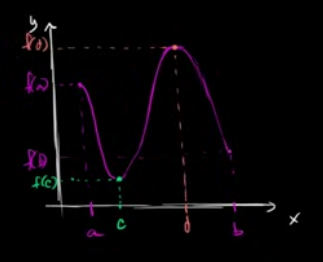
\includegraphics[bb=0 0 323 262, width=0.7\textwidth]{images/minimum_maximum.png}
            \caption{secant line}\label{fig:minimum_maximum}
        \end{figure}
         \[\exists\  c, d \in [a, b] : f(c) \le f(x) \le f(d)\ \forall\ x \in [a,b] \]
     \subsection{Critical points introduction}
        let \(x_0\), \(x_1\), \(x_2\) be non endpoints  maximum or minimum points of \(f(x)\), then the derivative of \(f'(x_0)\), \(f'(x_1)\), \(f'(x_2)\) is either going to be 0 or undefined.\\ 
        A critical point is a point where \(f'\) is equal to 0 or undefined.\\ 
        A critical point is not necessarily an extreme point, the reverse is true.
\section{Determining intervals on which a function is decreasing or increasing}
    \subsection{Increasing and decreasing intervals}
        The intervals where a function \(f(x)\) is increasing (or decreasing) correspond to the intervals where its derivative is positive (or negative) \(f'(x) < 0\) or \(f'(x) > 0\). \\ 
        the derivative of function changes sign at each critical point. 
\section{Using the first derivative test to find  relative (local) extrema}
    \subsection{first derivative test}
        If \(a\) is  min/max value of \(f(x)\) at \(x = a\) then \(a\) is a critical point.\\
        If \(a\) is critical point and in the domain of definition of f.then \(a\) is a maximum point of \(f(x)\), if \(f'(x)\) switches sign from positive to negative as \(f'(x)\) cross \(x = a\).\\  
        If \(a\) is a critical point and in the domain of definition of f.then \(a\) is a minimum point of \(f(x)\), if \(f'(x)\) switches sign from negative to positive as \(f'(x)\) cross \(x = a\). 
        \begin{figure}[ht]
            \centering
            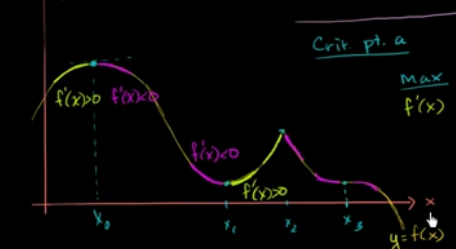
\includegraphics[bb=0 0 456 249, width=0.7\textwidth]{images/first_derivative_test.png}
            \caption{secant line}\label{fig:first derivative test}
        \end{figure}
\section{Using the candidates test to find absolute (global) extrema}
    \subsection{Absolute minima and maxima}
        let \(f(x)\) be defined function over the interval  \(x \in [a, b]\).\\ 
        let \(x_0\), \(x_1\) \(x_2\) be critical points and maximum points of \(f(x)\), where \(f'(x_0) = 0 \ | \ undefined\), \(f'(x_1) = 0 \ | \ undefined\), \(f'(x_2) = 0 \ | \ undefined\).\\
        \(x_1\) is an absolute maximum of \(f(x)\) if and only if \(f(x_1) > f(x_0)\ and \ f(x_1) > f(x_2)\ and \ f(x_1) > f(a)\ and \ f(x_1) > f(b)\).\\
        let \(x_0\), \(x_1\) \(x_2\) be critical points and minimum points of \(f(x)\), where \(f'(x_0) = 0 | undefined\), \(f'(x_1) = 0 | undefined\), \(f'(x_2) = 0  | undefined\).\\
        \(x_1\) is an absolute minimum of \(f(x)\) if and only if \(f(x_1) < f(x_0)\ and \ f(x_1) < f(x_2)\ and \ f(x_1) < f(a)\ and \ f(x_1) < f(b)\).
\section{Determining concavity of intervals and finding points of inflection}
        \subsection{Concavity introduction}
            let \(f(x)\) be  continuous and defined over the interval \([a,b]\).\\ 
            \(f(x)\) is concave downards on a sub interval of \([a,b]\) and has maximum point at \(x_0\) where \(f'(x_0) = 0\) iff: 
            \begin{itemize}
                \item  slope is decreasing: \(f'(x)\) is decreasing
                \item  the second derivative is negative: \(f''(x) < 0 \)
            \end{itemize}
            \(f(x)\) is concave upwards on a sub interval of \([a,b]\) and has minimumpoint at \(x_0\) where \(f'(x_0) = 0\) iff: 
            \begin{itemize}
                \item  slope is increasing: \(f'(x)\) is increasing
                \item  the second derivative is positive: \(f''(x) > 0 \)
            \end{itemize}
            \begin{figure}[ht]
                \centering
                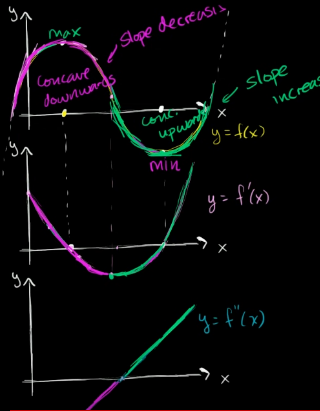
\includegraphics[bb=0 0 320 411, width=0.7\textwidth]{images/concavity.png}
                \caption{secant line}\label{fig:concavity}
            \end{figure}
        \subsection{Inflectoin point introduction}
            Inflection points is a point where the second derivative switches signs \\
            \(x_1\) is an inflection point iff: 
            \begin{itemize}
                \item for \(x < x_1 \): \(f''(x) < 0\) and for \(x > x_1\): \(f''(x) > 0\)
                \item or for \(x < x_1 \): \(f''(x) > 0\) and for \(x > x_1\): \(f''(x) < 0\) 
            \end{itemize}
\section{Second derivative test}
            let \(f'(c) = 0\), \(f'\) exists in neighborhoud around \( x = c\) \\ 
            let \(f''(c)\) exists then \\
            \begin{itemize}
                \item if \(f''(c) < 0\) then \(f\) has  relative maximum at \(x = c\)
                \item if \(f''(c) = 0\) then \(x = c\) is inconclusive 
                \item if \(f''(c) > 0\) then \(f\) has  relative minimum at \(x = c\)
            \end{itemize}
            
\section{Exploring accumulations of change }
        \subsection{Intro to integral calculus}
            let \(f(x)\)  be a  defined function.\\ 
            let \(\delta x_i\) be an infinitesimally small distance of the interval \([a, b]\). \\ 
            the area under the curve of \(f(x)\) between the interval \([a, b]\)
            is represented as: 
                \[\lim_{n \to \infty } \sum_{i=1}^{n} f(x_i) \delta x_i = \int_{a}^{b} f(x)dx\] 
            \(\int_{a}^{b}\) represents the integral of the function \(f(x)\)

            \begin{figure}[ht]
                \centering
                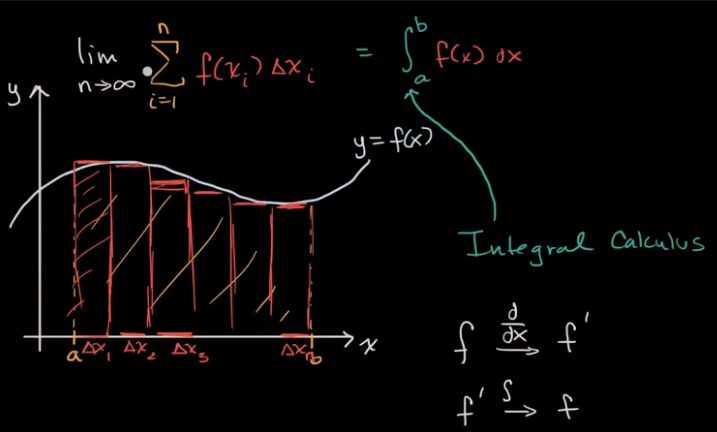
\includegraphics[bb=0 0 717 432, width=0.7\textwidth]{images/intro_integral.png}
                \caption{integrals}\label{fig:integral}
            \end{figure}
        \subsection{Definite integrals intro}
            The area under the curve between the interval \([a,b]\) is denoted as: 
                 \[\int_{a}^{b} f(x)dx\]
            which is the definite integral of \(f(x)\) between two bounds.
        \subsection{Exploring accumulations of change}
            The definite integral can be used to express information about accumulation and net change in applied contexts.
            the definite integral always gives us the net change in a quantity, not the actual value of that quantity\\
            In differential calculus, the derivative \(f'\) of a function \(f\) gives the instantaneous rate of change of \(f\) for a given input.\\
            for any rate function \(f\), its antiderivative \(F\) gives the accumulated value of the quantity whose rate is described by \(f\).\\\\
            \begin{center}
                \begin{tabular}{ c c c } 
                    & Quantity & Rate \\
                    \\
                    \multirow{1}{10em}{Differential calculus } & \(f(x)\) & \(f'(x)\) \\\\ 
                    \multirow{1}{10em}{Integral calculus} & \(F(x) = \int_{a}^{x}f(t)dt\) & \(f(x)\) \\ 
            
                    
                \end{tabular} 
            \end{center}
    \section{Approximating areas with Riemann sums}
        \subsection{RRiemann approximation introduction}
            A Riemann sum is an approximation of the area under a curve by dividing it into multiple simple shapes (like rectangles or trapezoids).\\\\
            In a left Riemann sum, we approximate the area using rectangles (usually of equal width), where the height of each rectange is equal to the value of function at the left endpoint of its base, this type of approximation is considered underestimate.\\
            \begin{figure}[ht]
                \centering
                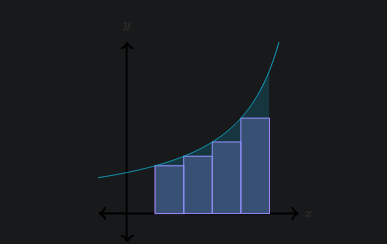
\includegraphics[bb=0 0 387 244, width=0.7\textwidth]{images/left_riem.png}
                \caption{integrals}\label{fig:left Reimann}
            \end{figure} \\ \\
            In a right Riemann sum, the height of each rectangle is equal to the value of the function at the right endpoints of its base.this type of approximation is considered overestimate\\
            \begin{figure}[ht]
                \centering
                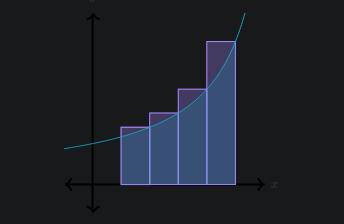
\includegraphics[bb=0 0 355 244, width=0.75\textwidth]{images/right_riem.png}
                \caption{integrals}\label{fig:right Reimann}
            \end{figure} \\
            In a midpoint Riemann sum, the height of each rectangle is equal to the value of the function at the midpoint of its base.\\
            \begin{figure}[ht]
                \centering
                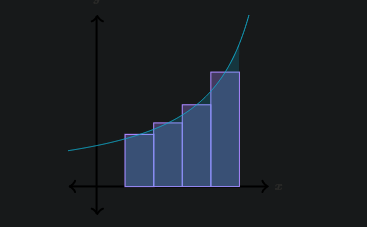
\includegraphics[bb=0 0 355 244, width=0.75\textwidth]{images/mid_riem.png}
                \caption{integrals}\label{fig:midpoint Reimann}
            \end{figure} \\
            We can also use trapezoids to approximate the rea (this is called trapezoidal rule). In this case, each trapezoid touches the curve at both of its top vertices.\\
            \begin{figure}[ht]
                \centering
                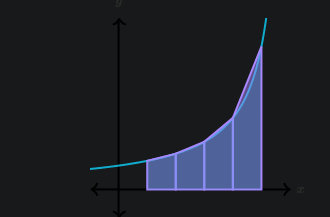
\includegraphics[bb=0 0 355 244, width=0.75\textwidth]{images/trap_rule.png}
                \caption{integrals}\label{fig:trapezoid rule}
            \end{figure} \\
        \section{Riemann sums, summation notation and definite integral notation}
            \subsection{Riemann sums in summation notation}
                Imagine we want to approximate the area under the graph of f over the interval \([a,b]\) with \(n\) equal subdivisions.\\
                Define \(\delta x\): let \(\delta x\) denote the width of each rectangle, then \(\delta x = \frac{b - a}{n}\)\\
                Define \(x_i\): Let \(x_i\) denote the right endpoint of each rectangle, then \(x_i = a + \delta x \cdot i \).\\ 
                Define the area of \(i^{th}\): The height of each rectangle is then \(f(x_i)\), and are of each rectangle is \(\delta x \cdot f(x_i)\).\\
                sum the rectangles: Now we use summation notation to add all the areas. The values we use for i are different for left and right Riemann sums: 
                \begin{itemize}
                    \item When we are writing a right Riemann sum, we will take values of \(i\) from 1 to \(n\)
                    \item However, when we are writing a left Riemann sum, we will take values of \(i\) from 0 to \(n - 1\)(this will give us the value of \(f\) at the left endpoint of each rectangle). 
                \end{itemize}
                \begin{center}
                    \begin{tabular}{ c c  } 
                        Left Riemann sum & Right Riemann sum  \\
                        \\
                        \(\sum_{i=0}^{n-1} \delta x \cdot f(x_i)\) & \(\sum_{i=1}^{n} \delta x \cdot f(x_i)\) \\\\ 
                       
                
                        
                    \end{tabular} 
                \end{center}
            \subsection{Definite integral as the limit of a riemann sum}
                The definite integral of a continuous function \(f\) over the interval \([a,b]\), denoted by \(\int_{a}^{b} f(x)dx\), is the limit of a Riemann sum as the number of subdivisions approches infinity.that is, 
                \[\int_{a}^{b} f(x)dx = \lim_{n \to \infty} \sum_{i = 1}^{n} \delta x \cdot f(x_i)\]

                where  \(\delta x = \frac{b - a}{n}\) and \(x_i = a + \delta x \cdot i\)
        \section{The fundamental theorem of calculus and accumulation functions}
                \subsection{the fundamental theorem of calculus}
                    let \(f\) be continuous function over the interval \([a, b]\).\\ 
                    let \(F(x) = \int_{a}^{x} f(t)dt\), where \(x\) is in \([a,b]\).\\
                    the fundamental theorem of calculus states that: 
                    \[\frac{dF}{dx} = \frac{d}{dx}[\int_{a}^{x} f(t)dt]= f(x)\]
                    \begin{itemize}
                        \item Every continuous function \(f\) has an antiderivative \(F(x)\). 
                        \item the FTOC connects integration and differentiation
                        \item \(F(x)\) is an antiderivative of \(f\).
                    \end{itemize}
        \section{Applying properties of definite integrals}
                \subsection{Negative definite integrals}
                    let \(f\) be continuous defined function.\\ 
                    let \(f([a,b]) < 0\). 
                    then 
                        \[\int_{a}^{b} f(x)dx < 0\]
                \subsection{Definite integrals properties}
                    Sum/Difference: 
                        \[\int_{a}^{b}[f(x) \pm g(x)]dx = \int_{a}^{b} f(x)dx \pm \int_{a}^{b} g(x)dx\]
                    Constant multiple: 
                        \[\int_{a}^{b} k \cdot f(x)dx = k \int_{a}^{b} f(x)dx\]
                    Reverse interval: 
                        \[\int_{a}^{b} f(x)dx = - \int_{b}^{a} f(x)dx\]
                    Zero-length interval: 
                        \[\int_{a}^{a} f(x)dx = 0\]
                    Adding intervals: 
                        \[\int_{a}^{b} f(x)dx + \int_{b}^{c} f(x)dx = \int_{a}^{c} f(x)dx \]
        \section{The fundamental theorem of calculus and definite integrals II}
                \subsection{the fundamental theorem of calculus II}
                    let \(F(x) = \int_{c}^{x} f(t)dt\) and \(F'(x) = f(x)\). 
                    then 
                        \[F(b) - F(a) = \int_{c}^{b} f(t)dt - \int_{c}^{a} f(t)dt = \int_{a}^{b} f(t)dt\]
                    OR 
                        \[\int_{a}^{b} f(t)dt = F(b) - F(a)\]
                \subsection{Antiderivative and indefinite integrals}
                    The antiderivative of \(2x\) is \(\int 2x dx = x^{2} + c\).\\ 
                    ther term \(\int 2x dx \) is called an indefinite integral. 
                \subsection{Proof of the fundamental theorem of calculus}
                    let \(F(x) = \int_{a}^{x} f(t)dt\) where \(a \le x \le b\). 
                        \[F'(x) = \lim_{\delta x \to 0} \frac{F(x + \delta x) - F(x)}{\delta x} = \lim_{\delta x \to 0} \frac{\int_{a}^{x + \delta x} f(t)dt - \int_{a}^{x} f(t)dt }{\delta x} \] 
                        \[= \lim_{\delta x \to 0} \frac{1}{\delta x} \int_{x}^{x + \delta x} f(t) dt\]
                    according to the mean value theorem of definite integral, there exists  a c (where \(x \le c \le x + \delta x\)) such that: \[f(c)\delta x = \int_{x}^{x + \delta x} f(t)dt\]
                    \[f(c) = \frac{1}{\delta x}\int_{x}^{x + \delta x} f(t)dt\]
                    as consequence and according to the squeeze theorem: \\
                        \(c \to x  \) as \(\delta x \to 0\).\\ 
                        \(f(c) \to f(x)\) as  \(\delta x \to 0 \)
                            \[x \le c(\delta x) \le x + \delta x\]
                    \(\lim_{\delta x \to 0 } x = x\), \(\lim_{\delta x \to 0 } c(\delta x) = x\), \(\lim_{\delta x \to 0 } x + \delta x = x\)
        \section{Finding antiderivatives and indefinite integrals: basic rules and notation: reverse power rule}
                    \subsection{Reverse power rule}
                        \[\int x^{n}dx = \frac{x^{n + 1}}{n + 1} + c \]
                     where \(n \neq -1 \) and \(c\) is some constant. 
                     \subsection{Indefinite integrals: sum and multiples}
                        \begin{itemize}
                            \item \(\int[f(x) + g(x)]dx = \int f(x)dx + \int g(x)dx\)
                            \item \(\int c f(x) dx = c \int f(x)dx\).
                        \end{itemize}
        \section{finding antiderivative and indefinite integrals: basic rules and notation: common indefinite integrals}
                        \subsection{Polynomials}
                            \[\int x^{n} dx = \frac{x^{n + 1}}{n + 1} + c\]
                        \subsection{Radicals}
                            \[\int \sqrt[m]{x^{n}} dx = \int x^{\frac{n}{m}} dx\]
                            \[= \frac{x^{\frac{n}{m} + 1}}{\frac{n}{m} + 1} + c\]
                        \subsection{Trigonometric functions}
                            \[\int \sin (x) dx = -\cos (x) + c\]
                            \[\int \cos (x) dx = \sin (x) + c\]
                            \[\int \sec^{2} (x) dx = \tan (x) + c\]
                            \[\int \csc^{2} (x) dx = -\cot (x) + c\]
                            \[\int \sec (x) \tan (x) dx = \sec (x) + c\]
                            \[\int \csc (x) \cot (x) dx = -\csc (x) + c\]
                        \subsection{Exponential functions}
                            \[\int e^x dx = e^x + c\]
                            \[\int a^x dx = \frac{a^{x}}{\ln(a)} + c\]
                        \subsection{Integrals that are lograithmic functions}
                            \[\int \frac{1}{x} dx = \ln |x| + c\]
                        \subsection{Integrals that are inverse trigonometric functions}
                            \[\int \frac{1}{\sqrt{a^{2} - x^{2}}} dx = \arcsin (\frac{x}{a}) + c\]
                            \[\int \frac{1}{a^{2} + x^{2}} dx = \frac{1}{a} \arctan (\frac{x}{a}) + c\]
            \section{Integrating using substitution}
                        \subsection{u-substitution}
                            u-substitution is about reversing the chain rule: 
                                \begin{itemize}
                                    \item according to the chain rule, the derivative of \(w(u(x))\) is \(w'(u(x)) \cdot u'(x)\).
                                    \item In u-substitution, we take an expression of the form \(w'(u(x)) \cdot u'(x)\) and find its antiderivative \(w(u(x))\)
                                \end{itemize}
                            u-substitution helps us take an expression and simplify it b making the ``inner'' function the variable.
                            example: 
                                    \[\int 2x \cos(x^2)dx\]
                            where \(u(x) = x^2\) and \(w(x) = \cos(x)\) 
                            sometimes we need to multiply/divide the integral by a constant, to get the derivative of \(u(x)\).
                                ex: 

                                    \[\int \sin(3x + 5)dx = \frac{1}{3} \int \sin(3x + 5) 3dx\]

                        \subsection{u-substitution with definite integrals}
                                when performing u-substitution for definite integral we need to account for the limits of integration, ex: \\ 
                                let \(\int_{1}^{2} 2x{(x^{2} + 1)}^{3}dx\).\\
                                \(2x\) is the derivative of \(x^{2} + 1\), so \(u = x^2 + 1\) and \(du = 2x dx\). \\
                                    \[\int_{1}^{2} 2x{(x^{2} + 1)}^{3}dx = \int_{1}^{2} u^{3} du\]
                                since the integration limit are fitted for \(x\) when need to fit it for \(u\). \\ 
                                since \(u = x^2 + 1\) the new bounds will be: 
                                \begin{itemize}
                                    \item Lower bound: \({(1)}^2 + 1 = 2\)
                                    \item Upper bound: \({(2)}^2 + 1 = 5\)
                                \end{itemize}
                                     \[\int_{1}^{2} 2x{(x^{2} + 1)}^{3}dx = \int_{2}^{5} u^{3} du\]
                                alternative way: keep the limits of integration, but substitute back to x before calculating defninite integral, ex: 
                                    \[\int_{1}^{2} 2x{(x^{2} + 1)}^{3}dx\]
                                    \[ = \int_{x = 2 }^{x = 1} {(u)}^3du\]
                                    \[ = {[\frac{u^4}{4}]}^{x = 2}_{x = 1}\]
                                    \[ = {[\frac{(x^2 + 1 )}{4}]}^{x = 2}_{x = 1}\]
                                    \[ = \frac{{[(2^2 + 1 )]}^4}{4} - \frac{{[(1^2 + 1 )]}^4}{4}\]
                                    \[ = 152.25\]
               \section{Differential Equations} 
                         \subsection{Introduction}
                              A differential equation is an equation that elates one or more unknown functions and their derivatives. 
                               \[y'' + 2y' = 3y \]
                               \[f''(x) + 2f'(x) = 3f(x) \]
                               \[\frac{d^2 y}{d x^2} + 2 \frac{dy}{dx} = 3y \]
                               The solution to a differential equation is a function or a class of functions, 
                \section{Slope fields}
                          \subsection{Introudction}
                               A slope field is a graphical representation of the solutions to a first-order differential equation.
                               \begin{figure}[ht]  
                                \centering
                                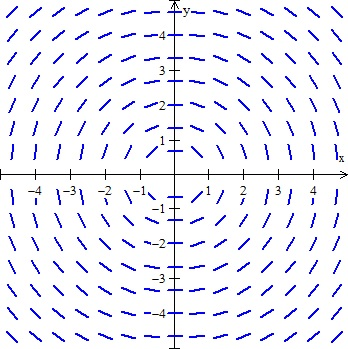
\includegraphics[bb=0 0 323 262, width=0.7\textwidth]{images/slope-field-1.jpg}
                                \caption{slope field}\label{fig:slope field}
                            \end{figure} 
                \section{Separable differential equation}
                        \subsection{Intro}
                            Separable differential equation: are equations that can be solved using separation of varibales.\\
                            To solve a differential equation using separatoin of varibales.we must be able to bring it to the form \(f(y)dy = g(x)dx\).\(f(y)\) is an expressoin that doesn't conatain \(y\).and \(g(x)\) is an expression that doesn't contain \(y\) 
                \section{Finding the average value of a function on an interval}
                    \subsection{Mean value theorem for integrals}
                        the average value of a function \(f\) over the interval \([a,b]\) is given as: 
                             \[\frac{\int_{a}^{b} f(x)dx}{b - a}\]    
                \section{Connecting position, velocity and acceleration functions using integrals}
                     \subsection{motion problems}
                            \begin{itemize}
                                \item  Displacement: `what is the particle's displacement between\ldots and\ldots ` or `What is the change in the particle's position between\ldots and\ldots ` \[\int_{a}^{b} v(t)dt\]
                                \item Total distance: `what is the total distance the particle has traveled between\ldots and\ldots ' \[\int_{a}^{b}|v(t)|dt\]
                                \item Actual position: `What is the particle's position at\ldots ` \[C + \int_{a}^{b}v(t)dt\]
                            \end{itemize}
                \section{Washer method} 
                            Washer method is a technique in calculus used for finding the volume of a solid or revolution when the solid has a hole in the middle, it's an extension of the disk method and it's used when you're rotating  a region aroun an axis and that region is bounded by two functions: an outer radius and an inner radius. 
                            \subsection{Formula round the x-axis}
                                if rotating around the x-axis,and the region is between  two curves \(y = R(x)\) (outer) and \(y = r(x)\) (inner) from \(x = a\) to \(x = b\) then the volume is: 
                                \[V = \pi \int_{a}^{b} [{R(x)}^2 - {r(x)}^2]dx\]
                                \begin{itemize}
                                    \item \(R(x)\): outer radius (from axis to outer curve)
                                    \item \(r(x)\): inner raius (from axis to inner curve)
                                \end{itemize}
                             \subsection{Formula about the y-axis (solve for x)}
                                \[V = \pi \int_{a}^{b} [{R(y)}^2 - {r(y)}^2]\]
                            \subsection{When to use washer method}
                                \begin{itemize}
                                    \item when rotating around a horizontal or vertical axis
                                    \item when region lies between two curves 
                                    \item solid has a hole in the middle
                                \end{itemize}
                \section{Disk Method}
                        the Disk method is a technique used to find thhe volume of a solid of revolution when a region is rotated around an axis
                        \subsection{Formula (rotating around x-axis)}
                            \[V = \pi \int_{a}^{b} [{R(x)}^2]dx\]
                            where: 
                            \begin{itemize}
                                \item \(R(x)\) is the radius of the disk (distance from the axis to the curve)
                                \item \(a\) to \(b\) are the limits of integration
                            \end{itemize}
                        \subsection{When to use disk method}
                            \begin{itemize}
                                \item the region is being rotated around the x-axis or the y-axis 
                                \item the solid has no hole in the middle 
                                \item the outer edge is defined by a single function 
                            \end{itemize}
                \section{Shell method}
                            shell method is a technique used to find the volume of a solid of revolution 
                            \subsection{shell method formula (about the y-axis)}
                                if a region between \(x = a\) and \(x = b\) is rotated about the y-axis the volume is: 
                                    \[V = 2\pi \int_{a}^{b} (radius \cdot height) dx\]
                                where: 
                                \begin{itemize}
                                    \item \(radius = distance from the axis of rotation \rightarrow x\)
                                    \item \(height = value of the function \rightarrow usually f(x)\)
                                \end{itemize}
                                shell method around x-axis: 
                                        \[V = 2\pi \int_{c}^{d} (radius \cdot height) dy\]
                            \subsection{when to use shell Method}
                            \begin{itemize}
                                \item When it's easier to integrate with respect to x, but the axis of rotation is vertical (like the y-axis).
                                \item When using the disk or washer method would require splitting the region into multiple parts or solving for inverse functions.
                            \end{itemize}
                \section{Integration by parts}
                            Integration by parts is used to find the integral of products: 
                            \[\int u(x)v'(x)dx = u(x)v(x) - \int u'(x)v(x)dx \]
                            \[\int u dv = uv - \int v du\]
                            this method is considred as the reverse power product rule.
                            \subsection{Using Liate rule to pick u}
                                \begin{table}[h!]
                                \centering
                                \begin{tabular}{lll}
                                \toprule
                                \textbf{Priority} & \textbf{Type} & \textbf{Example} \\
                                \midrule
                                L & Logarithmic      & \( \ln x \), \( \log_a x \) \\
                                I & Inverse Trig     & \( \tan^{-1}x \), \( \sin^{-1}x \) \\
                                A & Algebraic        & \( x \), \( x^2 \), \( x^3 \), etc. \\
                                T & Trigonometric    & \( \sin x \), \( \cos x \), \( \tan x \) \\
                                E & Exponential      & \( e^x \), \( 2^x \), \( a^x \) \\
                                \bottomrule
                                \end{tabular}
                                \caption{LIATE rule for choosing \( u \) in integration by parts}
                                \end{table}

                \section{Improper integrals}
                            Improper integrals are definite integrals that cover an unbounded area. \\ 
                            Two type of imporper integrals: 
                            \begin{itemize}
                                \item an integral where one of the endpoints is extended to infinity ex: 
                                    \[\int_{1}^{\infty} \frac{1}{x^2} dx\]
                                    which is viewed as: 
                                    \[\lim_{b \to \infty} \int_{1}^{b} \frac{1}{x^2} dx\]
                                \item an integral whose endpoints are finite, but the integrated funtion is unbounded at one (or two) of the endpoints ex:
                                        \[\int_{0}^{1} \frac{1}{\sqrt{x}} dx\]
                                        it can be viewed as the limit: 
                                        \[\lim_{a \to 0^+} \int_{a}^{1} \frac{1}{\sqrt{x} dx}\]
                            \end{itemize}
                            When the limit exists we say the integral is \textbf{converget}, and when it doesn't we say it's \textbf{divergent}.
                \section{Approximating solution using Euler's method differential equation}
                      let \(\frac{dy}{dx} = x  + y\) and \(f(1) = 2\).\\ 
                      \(f(3) \approx \)?\\ 
                      using Euler's method we chose step size of  \(\Delta x = 1\). \\ 
                      we let \(\frac{dy}{dx} = F(x, y) = x + y\) to calculate \(\Delta y\) so that 
                      \[\Delta y_{n+1} \approx y_n + \Delta y_n\]
                      Then use Euler's method to determine the next \(y\)-value. 
                      \[y_{n + 1} = y_n +\Delta y_n\]
                      We'll need to repeat the process-iterate-two times to find the desired value. \\ 
                      We are given  \((x_0, y_0)=(1,2)\), the starting point. Let \(n = 1\). 
                      \[x_1 = x_0 + \Delta x \rightarrow  x_1 = 1 + 1 = 2\]
                       \[y_1 = y_0 + \Delta y_0 \rightarrow y_1 = 2 + 3 \cdot 1 = 5\]
                       Thus \((x_1, y_1) = (2, 5)\). Now let \(n = 2\). 
                       \[x_2 = x_1 + \Delta x \rightarrow x_2 = 2 + 1 = 3\]
                       \[y_2 = y_1 + \Delta y_1 \rightarrow y_2 = 5 + 7 \cdot 1 = 12\]
                       So \(f(3) \approx 12\).
                \section{Logistic models with differential equations}
                    \begin{figure}[ht]  
                        \centering
                        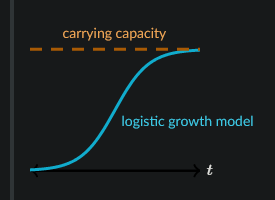
\includegraphics[bb=0 0 323 262, width=0.7\textwidth]{images/logistic_model.png}
                        \caption{slope field}\label{fig:logistic model}
                    \end{figure} 
                            \subsection{The logistic growth model}
                                let \(p\) be the population. 
                                the  rate of change of the population with respect to time is proportional to the population times \(1 - \frac{p}{k}\) where  \(k\) is the upper limit that the population can get and \(p = 0\) is the lowest limit the polpulatoin can get.\\
                                when the population at it's max limit k \(\frac{dp}{dt} = 0\). \\ 
                                the logistic differential equation is given as: 
                                \[\frac{dp}{dt} = rp(1 - \frac{p}{k})\]
                                Logistic growth mean initially growing almost exponentially, but the growth slows as the function approaches a horizontal asymptote.\\ 
                                In logistic growth, the carrying capacity is the upper limit the quantity grows towards \(\lim_{t \to \infty} P(t)\).\\
                                for any logistic model \(P\), the limit  \(\lim_{t \to \infty} \frac{dP}{dt} = 0\).\\ 
                                so  at the carrying capacity \(\frac{dP}{dt} = 0 \). 
                \section{Arc length}
                    let \(ds\) be small change in the arc length and \(dx, dy\) small change in \(x, y\) with respect to \(ds\).
                    the arc length over the interval \([a, b]\) is given as: 
                    \[\int ds = \int \sqrt{dx^2  + dy^2}\]
                    \[= \int \sqrt{dx^2 (1 + {(\frac{dy}{dx})}^2)}\]
                    \[\boxed{= \int_{a}^{b} \sqrt{1 + {(\frac{dy}{dx})}^2} dx}\]
                \section{Defining and differentiating parametric equations}
                    A parametric equation expresses coordinates (like x and y) as functions of a third variable, called a parameter (often represented by t) this is a way to define a curve or surface by describing how each coordinates changes with respect to the parameter. 
                    ex: \\
                    line \(x = at + b\), \(y = ct + d\) where a, b,c, and d are constants 
                    \subsection{Parametric equation differentiation}
                        to defferentiate a function that is defined parametrically by the equation \(x = u(t)\) and \(y = v(t)\).\space(where u and v are any function of t) we use the following rule: 

                        \[\frac{dy}{dx} = \frac{\left(\frac{dy}{dt}\right)}{\left(\frac{dx}{dt}\right)} = \frac{u'(t)}{v'(t)}\]
                \section{Second derivatives of parametric equations}
                    the second derivative is found with the following rule. 
                    \[\frac{d^2y}{dx^2} = \frac{\frac{d}{dt} (\frac{dy}{dx})}{(\frac{dx}{dt})} = \frac{\frac{d}{dt}(\frac{v'(t)}{u'(t)})}{u'(t)}\]
                \section{Parametric curve arc length}
                    Arc length of a parametric curve over the interval \([a, b]\): 
                    \[\int_{a}^{b} \sqrt{{(\frac{dx}{dt})}^2 + {(\frac{dy}{dt})}^2} dt = \int_{a}^{b} \sqrt{{u'(t)}^2 + {v'(t)}^2} dt\]
                \section{Defining and differentiating vector-valued functions}
                    A vector-valued function is a function that takes one or more variables as input and ouputs a vector.\\
                    General form in 2d: 
                    \[\vec{r}(t) = \langle x(t), y(t) \rangle \]                
                    or 
                    \[\vec{r}(t) = x(t)\hat{\imath} + y(t)\hat{\jmath}\]
                    \subsection{vector-valued functions differentiation}
                    the derivative of vvf is the derivative of it's compnents. 
                         \[\vec{r}  '(t) = \langle x'(t), y'(t) \rangle \] 
                \section{Solving motion prolbems using vvf}
                    the vvf of velocity is given as  
                    \[\vec{v}(t) = (\frac{dx}{dt}, \frac{dy}{dt})\]
                    the vvf of acceleratoin is given assume
                    \[\vec{a}(t)= \frac{d}{dt}\vec{v}(t) = (\frac{d^2x}{dt^2}, \frac{d^2y}{dt^2})\]
                    the magnitude of displacement is given as 
                    \[\sqrt{{(\Delta x)}^2 + {(\Delta y)}^2 }\]
                    where 
                    \[\Delta x = \int_{a}^{b} x(t)dt\]
                    \[\Delta y = \int_{a}^{b} y(t)dt\]
                \section{Defining polar coordinates and differentiating in polar form}
                    A polar function is defined using polar coordinates instead of cartesian (rectangular) coordinates.\\
                    polar coordinates: 
                    \begin{itemize}
                        \item r: the distance from the origin (called the pole)
                        \item \(\theta\): the angel from the positive x-axis (called the polar axis) measured in radians or degrees.
                    \end{itemize}
                     we write \((r, \theta)\) instead of \((x, y)\), polar function expresses r as a function of \(\theta\).
                     \[r = f(\theta)\] 
                     to convert between cartesian and polar: 
                     \begin{itemize}
                        \item  From polar to cartesian: \(x = r \cos{\theta}, y = r \sin{\theta}\)
                        \item from Cartesian to polar \(r = \sqrt{x^2 + y^2}, \theta = \arctan (\frac{y}{x})\)
                     \end{itemize}
                     polar function differentiation: 
                    \[\frac{d}{d\theta} y(\theta) = r(\theta)\sin{\theta}\]
                    \[\frac{d}{d\theta} x(\theta) = r(\theta)\cos{\theta}\]
                    \subsection{Formula for slope in polar coordinates}
                     \[\frac{dy}{dx} = \frac{r'\sin(\theta) + r\cos(\theta)}{r'\cos(\theta) - r\sin(\theta)}\]
                     \subsection{Polar area formula}
                        \[A = \frac{1}{2} \int_{\alpha}^{\beta} r{(\theta)}^2 d\theta\]
                     \subsection{General rule for finding \((\alpha , \beta)\)}
                        \begin{itemize}
                            \item A:find where the curve starts/ends. 
                                \begin{itemize}
                                    \item solve \(r(\theta) = 0\). 
                                    \item values of \(\theta\) are where the curve crosses the pole (origin). 
                                    \item they often serve as the bounds for on loop. 
                                \end{itemize}
                            \item B:look at symmetry 
                                \begin{itemize}
                                    \item many polar curves are symmetric. 
                                    \item symmetric about the x-axis \(\rightarrow\) integrate from 0 to \(\frac{\pi}{2}\) and multiply by 2. 
                                    \item symmetric about the y-axis \(\rightarrow\) integrate from 0 to \(\frac{\pi}{2}\) and multiply by 2. 
                                \end{itemize}
                            \item C:make sure \(r \geq 0 \)
                                \begin{itemize}
                                    \item if \(r(\theta)\) becomes negative, the curve is traced on the opposite side. 
                                    \item either adjust limits or take absolute value in the integral
                                \end{itemize}

                        \end{itemize}
                
                    \section{Convergent and divergent sequences}
                        A sequence \({a_n}\) converges to \(L\) if for every small number \(\beta > 0 \), there exists \(N\) such that for all \(n > N\), \(|a_n - L| < \beta\). \\
                        Examples: 
                        \begin{itemize}
                            \item \(\frac{1}{n} \rightarrow 0\)
                            \item \(\frac{2n}{n + 1} \rightarrow 2\)
                            \item \({(\frac{1}{n})}^2 \rightarrow 0\)
                        \end{itemize}

                        A sequence is divergent if it does not converge (diverge) to a finite number. \\ 
                        A sequence diverges when it: 
                        \begin{itemize}
                            \item Goes to infinity: \(a_n = n \rightarrow \infty\)
                            \item Oscillates without approaching a single value: \(a_n = {(-1)}^2\)
                        \end{itemize}
                        \subsection{Partial Sum}
                            The \(n\)-th partial sum of a series is the sum of the first \(n\) terms: \\
                                \[S_n = \sum_{k = 1}^{n} a_k = a_1 + a_2 + a_3 + \cdots + a_n\]
                            so 
                            \begin{itemize}
                                \item \(S_1 = a_1\)
                                \item \(S_2 = a_1 + a_2\)
                                \item \(S_3 = a_1 + a_2 + a_3\)
                            \end{itemize}
                            the sequence of partial sum \({S_n}\) tells us if the series converges or diverges: 
                            \begin{itemize}
                                \item if \(\lim_{n \rightarrow \infty} S_n = S \) (a finite number), then the series \(\sum a_n\) converges to \(S\).
                                \item if the limit does not exist (goes to \(\infty , -\infty\) or oscillates), the series diverges.
                            \end{itemize}
                         \subsection{Partial sum formula for common type of series}
                            Arithmetic series (linear sequence)\\ 
                            if \(a_k\) is arithmetic: 
                                \[a_k = a_1 + (k - 1)d\]
                            the partial sum is: 
                                \[S_n = \frac{n}{2}(2a_1 + (n - 1)d)\]
                            or equivalently: 
                                \[S_n = \frac{n}{2}(a_1 + a_2)\]
                            Geometric Series \\ 
                            if \(a_k\) is geometric: 
                                \[a_k = a_1r^{k-1}\]
                            the partial sum is: 
                                \[S_n = a_1 \frac{1 - r^n}{ 1 - r} , r \neq 1\]
                    \section{Working with geometric series}
                            let \(a_n\) be a gemoetric series, and let \(\sum_{k = 0}^{\infty} a_n(r^k) = \frac{a_1}{ 1 - r}\). \\ 
                            \(a_n\) converges iff \(|r| < 1\).
                    \section{nth-term divergence test}
                          if \(\lim_{n \to \infty} a_n \neq 0\) or does not exist, then the serie \(\sum_{n = 1}^{\infty} a_n\) diverges. 
                          \begin{itemize}
                            \item nth test can only prove divergence, never convergence
                            \item if \(\lim_{n \to \infty} a_n = 0\), the series might converge or diverge
                          \end{itemize} 
                    \section{Integral test}
                          let 
                                \[\sum_{n = 1}^{\infty} a_n\]
                          if \(a_n = f(n)\) where \(f(x)\) is: 
                          \begin{itemize}
                            \item continuous
                            \item positive
                            \item decreasing
                          \end{itemize}
                          for all  \(x \geq N\) (some starting point),\\ 
                          then: 
                          \(\sum_{n=1}^{\infty} a_n\) converges iff \(\int_{N}^{\infty} f(x)dx\) converges.
                    \section{Harmonic series and p-series}
                          \subsection{harmonic series}
                            the harmonic series is the infinte series 
                                \[\sum_{n=1}^{\infty} \frac{1}{n} = 1 + \frac{1}{2} + \frac{1}{3} + \cdots\]
                    
                            it's called harmonic because th terms are the reciprocals of the positive integers, which are related to the harmonic mean in  mathematics.\\ 
                            Key properties: 
                            \begin{itemize}
                                \item it is a p-series with p = 1
                                \item the harmonic series diverges, even though \(a_n \rightarrow 0\).
                            \end{itemize}  
                          \subsection{P-series}
                            A p-series is an infinite series of the form: 
                                    \[\sum_{n = 1}^{\infty} \frac{1}{n^p}\]  
                            where \(p > 0\) is a real number.\\ 
                            Convergence Test: 
                            the convergence depends entirely on the value of p: 
                            \begin{itemize}
                                \item if \(p > 1\), the series converges. 
                                \item if \(0 < p \leq 1\), the series diverges.
                            \end{itemize}
                    \section{Comparison tests for convergence}
                            let \(\sum a_n \) and \(\sum b_n\) with \(a_n \geq 0 \) and \(b_n \geq 0\) for all \(n\) (nonnegative terms).\\
                            The Test\\
                            if \(0 \leq a_n \leq b_n\) for all \(n\) (or for sufficiently large n)
                            \begin{itemize}
                                \item if \(\sum b_n\) converges, then \(\sum a_n\) also converges. 
                                \item if \(\sum a_n\) diverges, then \(\sum b_n\) also diverges. 
                            \end{itemize}
                        \subsection{Limit test comparison}
                            let \(\sum a_n \) and \(\sum b_n\)  where \(a_n > 0\) and \(b_n > 0\). 
                            let: 
                                \[L = \lim_{n \to \infty} \frac{a_n}{b_n}\]
                                \begin{itemize}
                                    \item if \(0 < L < \infty\), then both series either converge or diverge. 
                                    \item if \(L = 0\) and \(\sum b_n\) converges, then \(\sum a_n\) also converges
                                    \item if \(L = \infty\) and \(\sum b_n\) diverges, then \(\sum a_n\) also diverges.
                                \end{itemize}
                    \section{Alternating series test}
                                An alternating series is one where the signs of the terms switch between positive and negative: 
                                    \[\sum_{n = 1}^{\infty} {(-1)}^{n-1} b_n\]
                                    or 
                                    \[\sum_{n = 1}^{\infty} {(-1)}^{n} b_n\]
                                \subsection{the test} 
                                    the series 
                                    \[\sum {(-1)}^{n} b_n\]
                                    converges if BOTH of these condition hold: 
                                    \begin{itemize}
                                        \item \(b_{n+1} \leq b_n \) for all \(n\) (the terms are monotonically decreasing)
                                        \item \(\lim_{n \to \infty} b_n = 0\)
                                    \end{itemize}
                                    if both conditions are satisfied, the series converges.
                    \section{Taylor and Maclaurin polynomials}
                                \subsection{Taylor Polynomial (centered at a)}
                                    let \(f(x)\) be a function that is \(n\)-times differentiable at \(x = a\). 
                                    The Taylor polynomial of degree \(n\) centered at \(a\) is: 

                                        \[P_n(x) = f(a) + f'(a)(x - a) + \frac{f''(a)}{2!}{(x - a)}^{2} + \cdot + \frac{f^{(n)}(a)}{n!}{(x - a)}^{n}\]
                                    or in summation form: 
                                        \[P_n(x) = \sum_{k = 0}^{n} \frac{f^{(k)}(a)}{k!}{(x - a)}^k\]
                                
                                 \subsection{Maclaurin polynomial}
                                     the Maclaurin polynomial is just a special case of the Taylor polynomial with \(a = 0\).
                                        \[p_n(x) = f(0) + f'(0)x + \frac{f''(0)}{2!}x^2 + \cdot + \frac{f^{(n)}(0)}{n!} x^n\]
                                    Or equivalently: 
                                        \[p_n(x) = \sum_{k = 0}^{n} \frac{f^{(k)}(0)}{k!} x^k\]
                                 \subsection{Key point}
                                    \begin{itemize}
                                        \item Taylor polynomial approximates a function near a general point \(a\). 
                                        \item Maclaurin polynomial is just a Taylor polynomial centered at 0.
                                    \end{itemize}
                        \section{Largrange error bound} 
                                \subsection{Taylor polynomial remainder}
                                    if \(f\) is \((n + 1)\)-times differentiable at \(a\), the taylor polynomial of degree \(n\) around \(a\) is 
                                        \[T_n(x) = f(a) + f'(a)(x - a) + \frac{f''(a)}{2!}{(x - a)}^{2} + \cdot + \frac{f^{(n)}(a)}{n!}{(x - a)}^{n} \]
                                    Then,
                                        \[f(x)  = T_n(x) + R_n(x)\]
                                    where \(R_n(x)\) is the remainder term.\\ 
                                    Forms of the Remainder 
                                    \begin{itemize}
                                        \item Largrange's Form (most common in analysis)
                                            \[R_n(x) = \frac{f^{(n + 1)}(\beta)}{(n + 1)!} {(x - a)}^{(n + 1)}\]
                                            for some \(\beta\) between \(a\) and \(x\).
                                        \item Integral Form 
                                            \[R_n(x) = \frac{1}{n!} \int_{a}^{x} f^{(n + 1)}(t){(x - t)}^n dt\]
                                    \end{itemize}
                                \subsection{Lagrange error bound}
                                    is thestandard practical way to bound Taylor remainder. \\
                                    if \(f\) is \((n + 1)\)-tiems continously differentiable on an interval containing \(a\) and \(x\), then the Taylor remainder after degree \(n\) satisfies the lagrange form 
                                        \[|R_n(x)| \leq \frac{M}{(n+1)!} |x - a|^{n+1}\]
                                    where \(M\) is any constant with 
                                        \[M \geq \max_{t \subset I}|f^{(n + 1)}(t)\]
                        \section{Power series}
                                    A power series is an infinte series of the form 
                                        \[\sum_{n=0}^{\infty} c_n {(x - a)}^n\]
                                        where 
                                        \begin{itemize}
                                            \item \(c_n\) are coefficients 
                                            \item \(a\) is the center of the series
                                            \item x is the variable
                                        \end{itemize}
                                    \subsection{Convergence of a power series}
                                        for a given \(x\), the series may converge or diverge.\\ 
                                        There is always a radius of convergence \(R \geq 0\) such that: 
                                        \begin{itemize}
                                            \item The series converges for all \(| x - a| < R\)
                                            \item Diverges for all \(| x - a| > R\). 
                                            \item On the boundary \(| x - a| = R\), each case must be checked separately.
                                        \end{itemize}
                                    \subsection{Finding the radius of convergence}
                                        use the ration test or root test 
                                            \[R = \lim_{n \to \infty} | \frac{c_n}{c_n + 1}|\]
                                        or 
                                            \[\frac{1}{R} = \lim_{n \to \infty}\sup \sqrt[n]{|c_n|}\] 
                        \section{Finding Taylor or Maclaurin series for a function}
                                        \subsection{Function as a geometric series}
                                            A geometric series representation of a function is when a  function \(f(x)\) can be written in the form 
                                                \[f(x) = \sum_{n = 0}^{\infty}ar{(x)}^n\]
                                            where: 
                                            \begin{itemize}
                                                \item \(a\) is a constant 
                                                \item \(r(x)\) is an expression in \(x\) that plays the role of the ratio
                                                \item the series converges when \(|r(x)| < x\)
                                            \end{itemize}
                                            Most common Case\\ 
                                            the basic geometric series identity is 
                                                \[\frac{1}{1 - r(x)} = \sum_{n = 0}^{\infty} r{(x)}^n , |r(x)| < 1\]
                                            this is the formal definition of expanding functions as geometric series 
                                        \subsection{Power series  and Maclaurin expansions of common functions}
                                            \begin{itemize}
                                                \item Geometric series 
                                                        \[\frac{1}{ 1 - x} = \sum_{n = 0}^{\infty} x^n , |x| < 1\]
                                                \item Exponential function 
                                                        \[e^x = \sum_{n = 0}^{\infty} \frac{x^n}{n!}, R = \infty\]
                                                \item Sine Function 
                                                        \[\sin(x) = \sum_{n = 0}^{\infty} {(-1)}^n \frac{{x}^{(2n + 1)}}{(2n + 1)!}, R = \infty\]
                                                \item Cosine Function 
                                                        \[\cos(x) = \frac{n = 0}{\infty} {(-1)}^{n} \frac{x^{2n}}{(2n)!},R = \infty \]
                                                \item Natural Logarithm   
                                                        \[\ln(1 + x) = \sum_{n = 1}^{\infty} {(-1)}^{n + 1} \frac{x^n}{n}, |x| < 1, x \neq -1\]
                                                \item Arctangent 
                                                        \[\arctan(x) = \sum_{n = 0}^{\infty}{(-1)}^n \frac{{x}^{2n + 1}}{2n + 1}, |x| \leq 1\]
                                            \end{itemize}
                                        Note: \\ 
                                        when finding power series of function we use algebraic manipulation to derive the series, when finding Maclaurin series of a function we use the forumla for Maclaurin series, common function have the equal power serie and maclaurin series expansions. 
\end{document}